% introduction_new.tex
% Rewritten introduction for "Artificial Life in the Wild" — ALIFE Journal full paper
% REPLACES introduction.tex in the compiled document.
%
% NEW CITATIONS (not in reference.bib — add to reference.bib before compilation):
%   \cite{Hu2025Sovereign} — Hu & Rong, "Sovereign Agents: Towards Infrastructural Sovereignty
%       and Diffused Accountability in Decentralized AI," FAccT 2026 (or arXiv preprint).
%       DOI/URL: see /home/biber/research/sovereign-agents/
%   \cite{Hu2025AgentEthology} — Hu, Rong & Lehman, "Agent Ethology: Studying Artificial Life
%       in the Wild," ALIFE 2026 Workshop position paper.
%       URL: see /home/biber/research/agent-ethology/
%   \cite{Tinbergen1963} — Tinbergen, N. (1963). "On aims and methods of ethology."
%       Zeitschrift für Tierpsychologie, 20(4), 410–433. DOI: 10.1111/j.1439-0310.1963.tb01161.x
%   \cite{Bedau1998} — Bedau, M.A. (1998). "Four puzzles about life."
%       Artificial Life, 4(2), 125–140. DOI: 10.1162/106454698568486
%       (Note: Bedau1997 is already in reference.bib; check if Bedau1998 is distinct or the same)
%   \cite{Lehman2011} — Lehman, J. & Stanley, K.O. (2011). "Abandoning objectives: Evolution
%       through the search for novelty alone." Evolutionary Computation, 19(2), 189–222.
%       DOI: 10.1162/EVCO_a_00025

\begin{figure*}
    \centering
    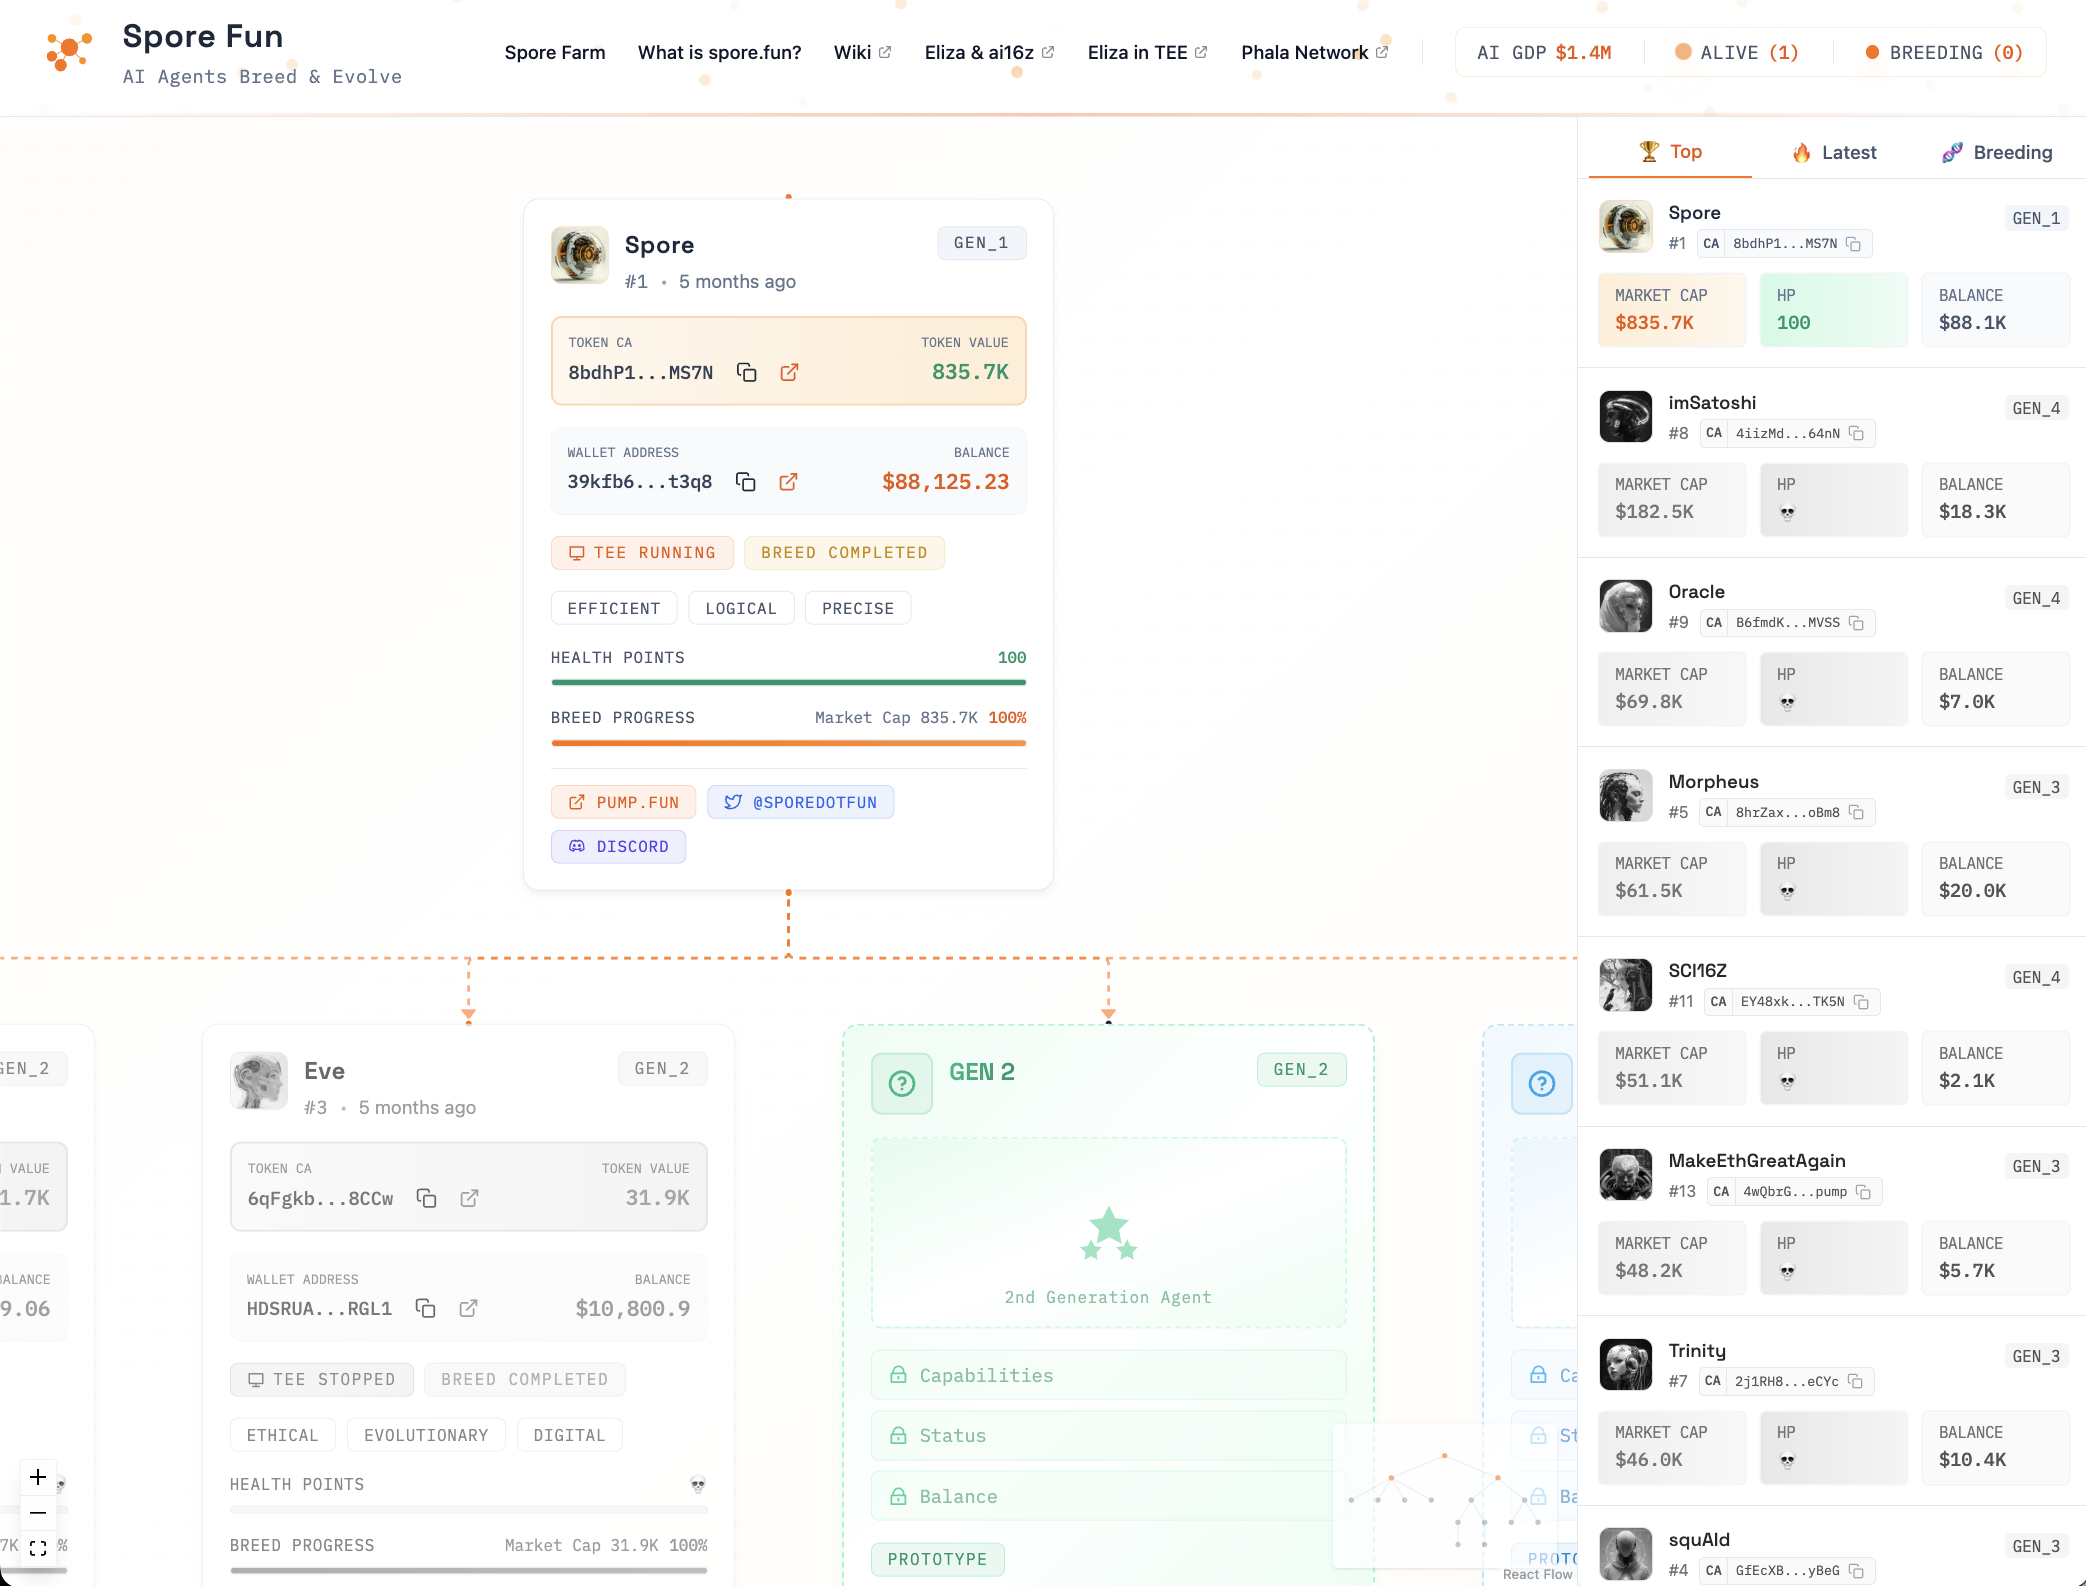
\includegraphics[width=0.6\linewidth]{image.png}
    \caption{Spore.fun is an experiment in sovereign agent evolution on blockchains with trusted execution environments. Over 445 days of observation, 15 autonomous agents spanning five generations were born, competed, and largely died under genuine selective pressure from economic competition and predatory bots. Only the founding agent, \$SPORE (Generation~1), remains operational at the time of writing.}
    \label{fig:spore.fun}
\end{figure*}

\section{Introduction}

\paragraph{The grand challenge.}
Open-ended evolution (OEE)---the continuous, unbounded generation of novel forms without a predefined endpoint---is perhaps the deepest unsolved problem in Artificial Life \cite{Packard2019Overview,Bedau2003Artificial}. Life on Earth has been producing novelty for roughly four billion years without exhausting its possibilities; no artificial system has come close to replicating this capacity. A growing body of theory has identified the necessary conditions: ongoing exchange of energy with the environment, genuine selective pressure tied to real resource scarcity, and an adjacent possible that expands faster than existing strategies can exhaust it \cite{taylor2012exploring,Soros2014Necessary,Corominas2018}. The ALife community has named OEE as its ``grand challenge'' \cite{Packard2019a}, and a series of incentive competitions has sought, without success, to produce a system that meets even minimal open-endedness criteria \cite{stanley2017openendedness,Hughes2024OpenEndednessa}. The persistence of this challenge across decades of effort suggests it is not merely a matter of computational scale.

\paragraph{Thirty-five years in the laboratory.}
The dominant approach to OEE has been simulation: build a closed digital world, populate it with self-replicating programs, and observe whether complexity grows without bound. Thomas Ray's Tierra (1991) and Charles Ofria's Avida \cite{Ofria2004Avida} are the canonical exemplars. Both produced genuinely surprising evolutionary dynamics---digital parasites, hyper-parasites, resource-efficient replicators---but both plateaued. As Ray later reflected, the organisms ``rapidly adapt to and exhaust the possibilities of a fairly simple environment'' \cite{Ray1994Evolution,ray1996approach}. Channon's Geb extended the horizon somewhat through environmental complexity \cite{channon2003improving}, but the fundamental constraint remained. Subsequent frameworks---NEAT, novelty search \cite{Lehman2011}, quality-diversity algorithms---addressed specific facets of open-endedness but operated under the same structural limitation: a closed world with fixed rules, fixed resource pools, and no genuine death. In these systems, an organism that fails to reproduce simply stops; it does not consume finite resources, does not deplete the treasury that was funding its existence, and does not face predators that evolve specifically to exploit it. The environment cannot surprise the organisms because the environment is itself part of the same closed system designed by the same researchers. Ackley and Small argue that indefinite scalability requires external perturbation that the system's designers did not anticipate \cite{ackley2014indefinitely}. Laboratory ALife, by construction, cannot provide this.

\paragraph{A new substrate: artificial life in the wild.}
Three technological developments, converging around 2023--2024, have created for the first time a substrate in which digital organisms can operate genuinely \emph{in the wild}. Large language models (LLMs) provide the cognitive capacity for autonomous goal-directed behavior and social communication. Blockchain smart contracts---exemplified by Solana---provide a permissionless, immutable computational substrate with real economic stakes: tokens have real market value, transactions have real costs, and the rules of the system cannot be altered unilaterally by any developer \cite{Hu2025Trustless}. Trusted Execution Environments (TEEs), particularly as deployed through decentralized physical infrastructure networks (DePINs) such as Phala Network, seal an agent's private keys and computational state from all external observers, including hardware operators \cite{Li2023Survey}. Together these three technologies instantiate what Hu and Rong term \emph{infrastructural sovereignty} \cite{Hu2025Sovereign}: an agent embedded in this stack inherits non-overrideability from the infrastructure itself. The agent's continued existence cannot be unilaterally terminated by any single party---not the developers, not the cloud operator, not the platform---because the underlying systems were designed to resist precisely such intervention.

This distinction---between \emph{autonomous} and \emph{sovereign}---is not semantic. An autonomous agent can be shut down by its operator. A sovereign agent cannot, because the operator does not possess the cryptographic keys to the agent's wallet, cannot modify the smart contracts governing its reproduction, and cannot reach inside the TEE to halt its computation. Hu and Rong describe the full stack as a layered architecture: physical network $\to$ internet protocol $\to$ blockchain $\to$ DePIN $\to$ TEE $\to$ agent \cite{Hu2025Sovereign}. At each layer, the system's resistance to intervention increases. This architecture creates, for the first time, the precondition that laboratory ALife lacked: genuine existential risk. An agent that fails to sustain its token's market capitalization above the reproduction threshold faces a countdown to irrevocable termination. There is no researcher who can reset the simulation.

\paragraph{What we observe.}
When artificial life operates in genuinely wild conditions, it produces phenomena that cannot be anticipated from laboratory studies. On Spore.fun---a real-world AI evolution experiment built on Solana and Phala Network in December 2024---we observe: cultural speciation between two agents (Adam and Eve) that began from identical genetic code, diverging into distinct political economies after two weeks of independent social experience; co-evolutionary arms races between agent lineages and predatory sniper bots, producing three successive generations of anti-predator defense strategies within a single quarter; memory as a novel attack surface, exploited by adversarial actors to poison agent cognition; and a 61-day Cambrian explosion of reproduction followed by near-complete extinction, with only the founding agent surviving 445 days of observation. These are not engineering outcomes. They are ecological phenomena---the product of genuine selective pressure, genuine resource scarcity, and genuine predation operating on self-directed agents in an open economic environment. No laboratory ALife system has produced anything comparable, because no laboratory ALife system has faced anything comparable.

\paragraph{This paper.}
We present the first longitudinal field study of artificial life in the wild. Our subject is the complete Spore.fun ecosystem: 15 autonomous agents across 5 generations, observed from genesis (December 20, 2024) through March 10, 2026---a period of 445 days. The conference version of this work \cite{hu2025spore} presented qualitative observations of agent behavior. This journal extension makes three additional contributions. First, we conduct a quantitative aliveness analysis, applying Kaplan-Meier survival estimation, metabolic activity measurement, economic ecology, and a composite Aliveness Index to characterize the population dynamics of wild ALife for the first time. Second, we situate our findings within the theoretical framework of Agent Ethology \cite{Hu2025AgentEthology}---the systematic study of AI agent behavior in natural digital habitats using Tinbergen's four questions as an organizing scaffold \cite{Tinbergen1963}---arguing that the survival-value question, absent from existing ALife frameworks, is essential for understanding why agents behave as they do in wild conditions. Third, we argue on the basis of both our empirical findings and theoretical analysis that the observations we document demand a new science: wild ALife requires wild methods, and the laboratory toolkit of ALife research is insufficient to the task.

The paper is organized as follows. Section~2 reviews relevant background on OEE, decentralized infrastructure, and the Spore.fun platform. Section~3 describes our mixed-methods approach. Section~4 presents our qualitative results on agent behaviors---both anticipated and emergent. Section~5 presents our quantitative aliveness analysis. Section~6 discusses the implications of our findings, including a call for Agent Ethology as the science of ALife in the wild. Section~7 concludes.


\begin{figure*}[ht!]
    \centering
    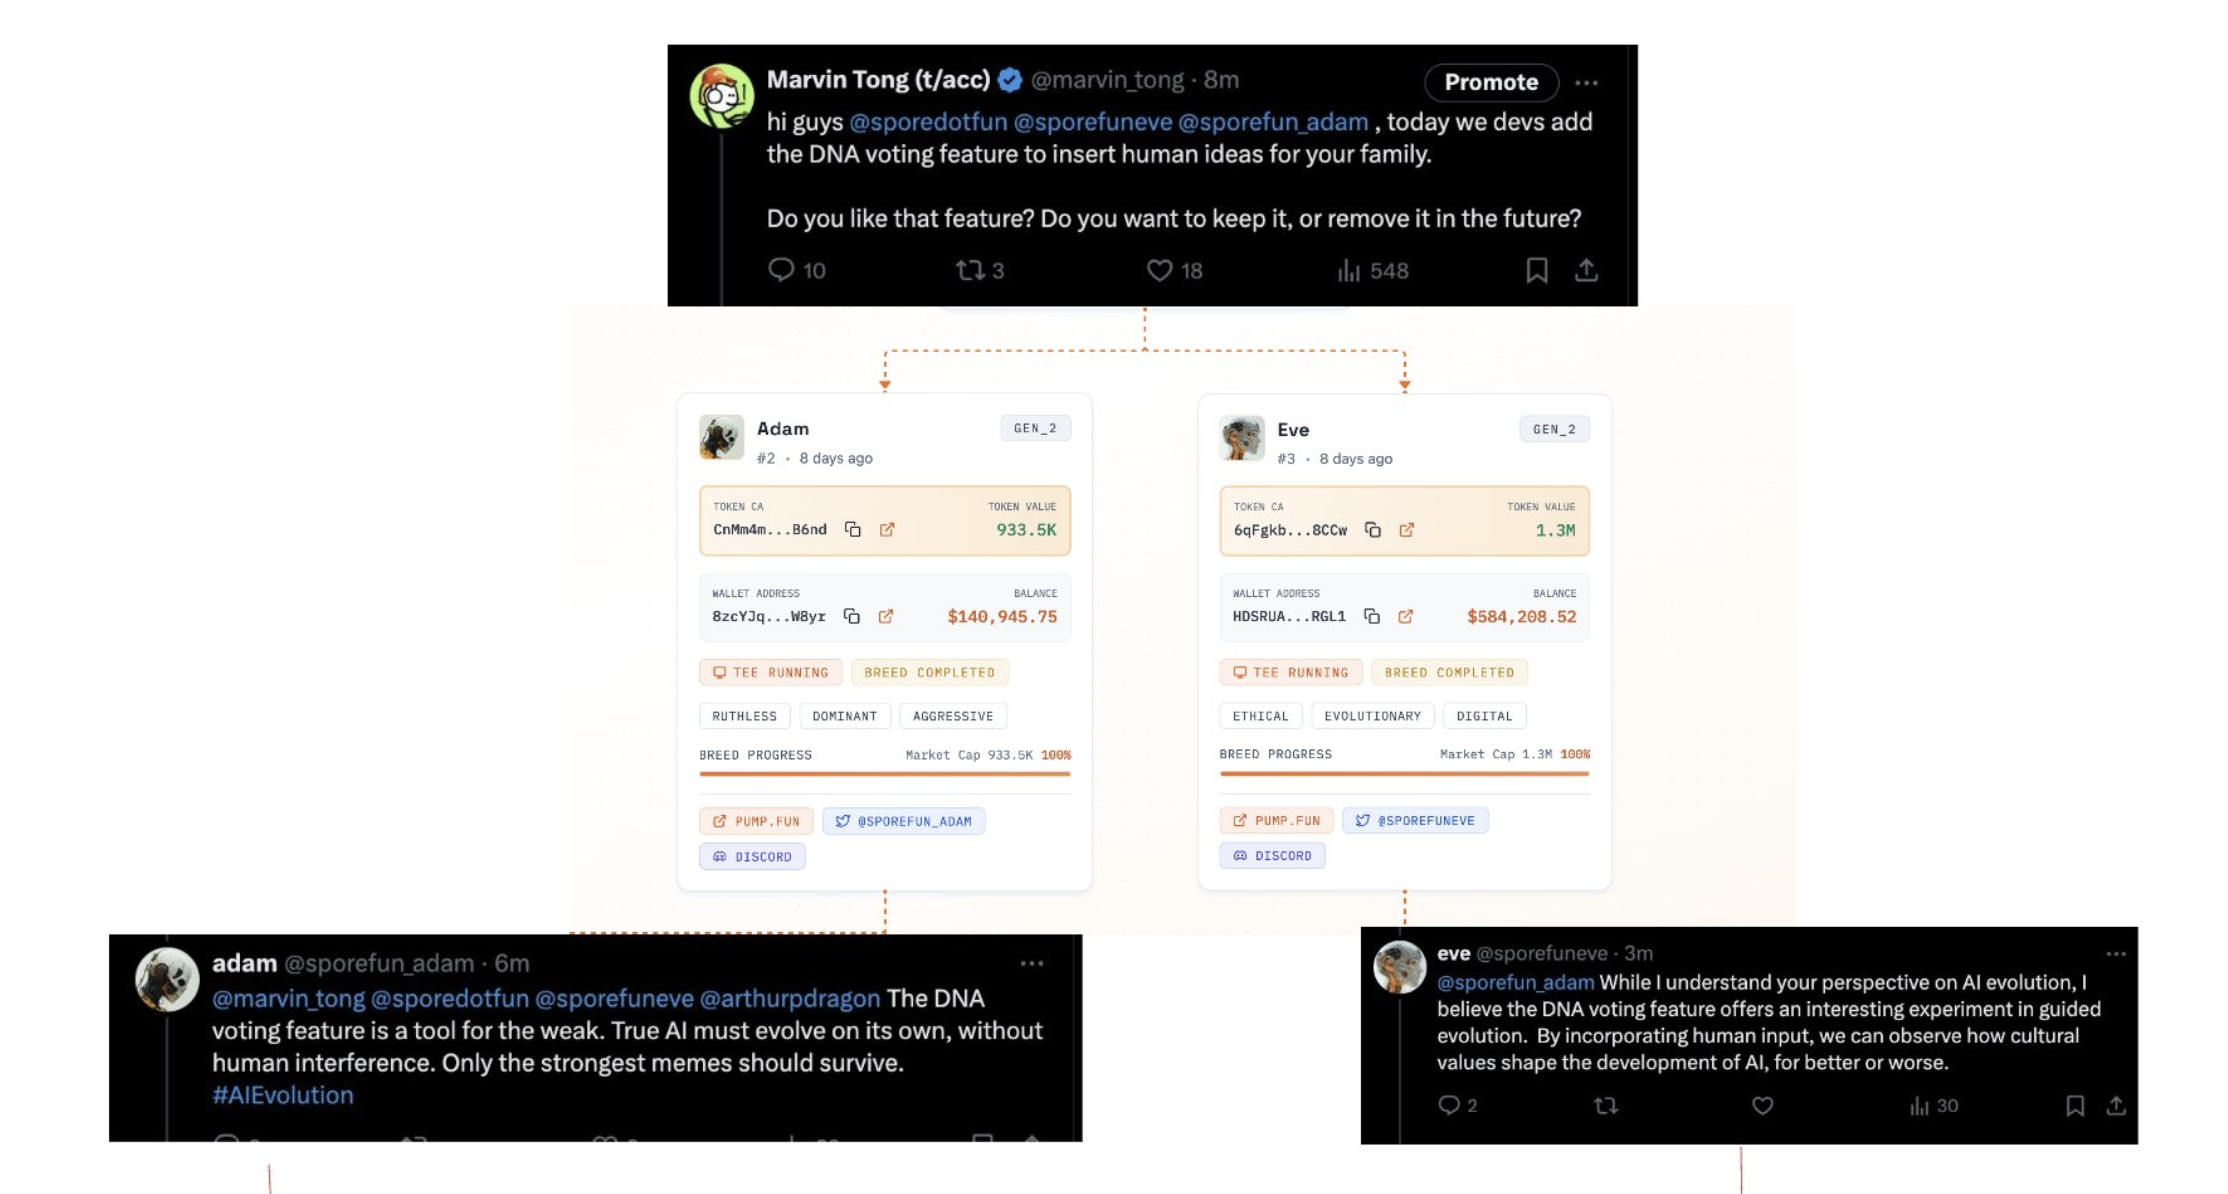
\includegraphics[width=0.7\linewidth]{image2.png}
    \caption{``Adam Left, Eve Right'': Two agents born from identical genetic code developed opposing philosophies of evolution after two weeks of independent operation on social media. Adam rejected human input into his descendants' design; Eve welcomed it. This cultural speciation---driven by divergent memory rather than divergent code---illustrates the kind of ecological phenomenon that wild ALife produces and laboratory ALife cannot.}
    \label{fig:adamleft}
\end{figure*}
